\expandafter\ifx\csname ifdraft\endcsname\relax
 \begin{document}
\fi

\section{方法}
\label{sec:method}

\subsection{換気量(V_E)}

製作する装置で測定する酸素摂取量VO_2, 呼気中二酸化炭素量VCO_2は1分あたりの量を表す

\subsubsection{換気量の測定}

\ref{sec:vo2}で示したように,換気量V_Eを測定するためには呼気量を測れば良い.



\subsubsection{STPD係数}
\label{sec:stpd}

呼気量から測定される換気量は,ATPS(Ambient Temperature, Pressure, Saturated with water vapor)においての値である.これは計測環境気温,計測環境気圧,水蒸気飽和における値である.酸素摂取量VO_2, 呼気中二酸化炭素量VCO2はSTPD(Standard Temperature, Pressure, Dry),0℃,1気圧の気体標準状態で表記されるため,ATPSをSTPDに換算する必要がある.この換算に使用する係数をSTPD係数と呼ぶ.STPD係数は以下の式で表される.

\begin{equation}
  \label{eq:stpd}
  STPD = \frac{P_B - P_{H2O}}{760} \times \frac{273.15}{273.15 + T}
\end{equation}

ただし,P_B: 気圧,P_{H2O}: 飽和水蒸気圧(\ref{sec:swvp}で記述する),T: 気温,273.15: 絶対温度である.

\subsubsection{飽和水蒸気圧}
\label{sec:swvp}

飽和水蒸気圧P_{H2O}は温度によって変化し,Tetens(1930)の式を用いて近似値を求めることができる.温度T[℃]の時の飽和水蒸気圧e(T)[mmHg]は次の式で求められる.

\begin{equation}
  e(T) = 6.1078 \times 10 ^ \frac{7.5T}{(T + 237.3)} \times \frac{760}{1013.25}
\end{equation}

\subsubsection{換気量の計算}

VO_2, VCO_2に使用される換気量は1分間値であるので,換気量V_{ATPS}を求めるためには呼気量Vを採気時間T[min]で割る.

\begin{equation}
  V_{ATPS} = \frac{V}{T}
\end{equation}

これにSTPD係数(\ref{eq:stpd})を掛けると換気量V_{STPD}が得られる.

\begin{equation}
  V_{STPD} = V_{ATPS} \times STPD
\end{equation}

\subsection{酸素摂取量}

酸素摂取量VO_2は単位時間あたり(多くの場合1分間値が用いられる)に身体に取り入れられた酸素の量を表す値である.よって,吸気中酸素量V_IO_2と呼気中酸素量V_EO2の差が酸素摂取量となる.吸気中酸素量,呼気中酸素量は,それぞれ吸気中酸素濃度F_IO_2と呼気中酸素濃度F_EO_2を用いて式\ref{eq:vo2formula}のように表せる.

\begin{equation}
  \label{eq:vo2formula}
  VO_2 = (V_I \times F_IO_2) - (V_E \times F_EO_2)
\end{equation}

よって,酸素摂取量は吸気中酸素量と呼気中酸素量を測定することにより求められる.しかし,実際には呼気の分析のみで酸素摂取量を求める方法が用いられる.

\subsubsection{窒素補正}
\label{sec:vo2fromvn2}

呼気の分析のみで酸素摂取量を求めるためには,{\bf 窒素は代謝に使われないため,身体に吸収されない}という性質を利用する.この性質から,吸気中窒素濃度F_IN_2と呼気中窒素濃度F_EN_2を用いて式\ref{eq:vin2ven2}が成り立つ.

\begin{equation}
  \label{eq:vin2ven2}
  V_I \times F_IN_2 = V_E \times F_EN_2
\end{equation}

V_Iに関してまとめると,V_Iは式\ref{eq:vi}のように表せる.

\begin{equation}
  \label{eq:vi}
  V_I = \frac{V_E \times F_EN_2}{F_IN_2}
\end{equation}

これを式\ref{eq:vo2formula}に代入すると次のようになる.

\begin{equation}
  \label{eq:vo2ve}
  VO_2 = \frac{V_E \times F_EN_2}{F_IN_2} \times F_IO_2 - V_E \times F_EO_2
\end{equation}

式\ref{eq:vo2ve}の右辺から,V_Eを括り出すことで次の式が成り立つ.

\begin{equation}
  \label{eq:getvo2fromn2}
  VO_2 = V_E \times (\frac{F_EN_2}{F_IN_2} \times F_IO_2 - F_EO_2)
\end{equation}

呼気中窒素濃度は呼気中酸素濃度と呼気中二酸化炭素濃度を100\%から引いた残りであるから,
式\ref{eq:getvo2fromn2}のF_EN_2はF_EO_2とF_IO_2を用いて式\ref{eq:fen2byfeo2feco2}のように表せる.

\begin{equation}
  \label{eq:fen2byfeo2feco2}
  VO_2 = V_E \times (\frac{100 - F_EO_2 - F_ECO_2}{F_IN_2} \times F_IO_2 - F_EO_2)
\end{equation}

通常大気中において,吸気中窒素濃度F_IN_2は79.04\%,吸気中酸素濃度F_IO_2は20.93\%であるから,これらを代入して式\ref{eq:fen2byfeo2feco2}は次のようになる.

\begin{equation}
  \label{eq:asdkjf}
  VO_2 = V_E \times (\frac{100 - F_EO_2 - F_ECO_2}{79.04} \times 20.93 - F_EO_2)
\end{equation}

式\ref{eq:asdkjf}から,呼気量V_Eと呼気中酸素濃度F_EO_2,呼気中二酸化炭素濃度F_ECO_2から酸素摂取量VO_2を求めることができる.

以上の式では,「窒素は代謝に使われないため,吸気と呼気中の窒素の量は変わらない」という特性を利用して,呼気中窒素量を用いて呼気中酸素量を補正することで吸気中酸素量を求めている.これを窒素補正という.

ただし,V_EはSTPD(Standard Temperature, Pressure, Dry),0℃,1気圧の気体標準状態である.ATPS(Ambient Temperature, Pressure, Saturated with water vapor)の呼気量からSTPDにおける換気量を計算するための係数,STPD係数を求める方法については\ref{sec:stpd}で述べる.

\subsection{呼気中二酸化炭素量}

呼気中二酸化炭素量VCO_2は単純に,STPD(\ref{sec:stpd})における換気量V_Eと呼気中二酸化炭素濃度を掛けて求めることができる.式は以下のようになる.

\begin{equation}
  \label{eq:vco2}
  VCO_2 = V_E \times (\frac{100 - F_EO_2 - F_ECO_2}{79.04} \times 20.93 - F_EO_2)
\end{equation}

\subsection{直接法と間接法}

\subsubsection{直接法}

人体で消費されたエネルギーは熱となって放射される.その熱量を直接測るのが直接法である.例えば,直接法の測定機器であるAtwater-Benedict-Rosa calorimeterでは,測定室内の被験者が放射する熱を室内に張り巡らされた管を流れる水の温度から測定する.それに加え,室内で発生した水蒸気量呼気などの水蒸気の気化熱を測定するとともに,測定中の体温の変化も考慮して,被験者のエネルギー消費量を測定する\cite{tanaka_2006}.

このように装置が大掛かりで,活動内容も測定室内で行えるものに限られるため,現在でも使用は一部の実験施設などに限られている.

\subsubsection{間接法}

そこで,測定が容易な別の値から間接的に消費エネルギーを求める方法が考案されてきた.中でも心拍数を用いて消費エネルギーを推定する方法は古くからRMR法などの方法が用いられ\cite{usutani_1990},現在では様々なデバイスやサービスで利用することができる.

しかし,心拍数は同一の被験者においても気温や体調によるばらつきが大きく,これを用いた消費エネルギーの推定は精度面で問題が残る.そこで,直接法ほど大掛かりな装置を用いずにより正確に消費エネルギーを推定する方法として,呼気分析によって消費エネルギーを推定する方法がある.

\subsection{Weirの式}
人体がエネルギーを生み出す際の化学反応から消費エネルギーを推定することができる.食物から取り込んだ栄養素が酸素と反応し,二酸化炭素を産出する.この化学式を用いて,酸素摂取量と二酸化炭素摂取量,尿素窒素量が正確に得られれば,エネルギー消費量が1\%もしくはそれ以下の誤差で推定できる\cite{livesey_1988}.

例えば,よく利用されるWeir\cite{weir_1949}の式は以下の通りである.

\begin{equation}
  \label{weir_urea_formula}
  EE(kcal) = 3.941 \times 酸素摂取量 + 二酸化炭素産生量 - 2.17 \times 尿中窒素排出量
\end{equation}

このうち,尿素窒素排出量は摂取エネルギーに閉めるたんぱく質の割合によって決まる.この値は比較的安定しており,たんぱく質の占める割合を12.5\%と仮定するとWeirの式は次のようになる.

\begin{equation}
  \label{weir_formula}
  EE(kcal) = 3.9 \times 酸素摂取量 + 1.1 \times 二酸化炭素産生量
\end{equation}

尿中窒素排出量を使用しないWeirの式は,たんぱく質の占める割合が20\%を大きく超えるような極端に偏った食事や,激しい運動中に限定したりすることをしなければ,誤差の影響は1\%未満であり,酸素摂取量と二酸化炭素産出量のみでも十分に正確に測定することができる\cite{tanaka_2006}.

呼気分析とWeirの式を用いた間接法は,直接法に比べて実施が容易である上に,心拍数などを用いた場合に比べてより精度の高い推定が可能である.それに加えて,呼気分析によって得られる酸素摂取量(VO2),呼吸回数(RR)及び換気量(VE)などの値は,アマチュアアスリートにとってもトレーニングや安全な運動のために有用なデータとなりうる.そこで,今回は呼気分析によって消費エネルギーを測定することができる呼吸代謝測定装置を製作する.

\subsection{計測項目}

\subsubsection{酸素摂取量(\.{V}_{O_2})と二酸化炭素産出量(\.{V}_{CO_2}),呼吸商}

酸素摂取量\.{V}_{O_2}は空気中の酸素(O_2)が単位時間(今回は慣例に従い1分間値とする)あたりにどれだけ身体に採り入れられたかを表す値である.よって,身体(肺)に採り入れた空気の量の大きさ(肺換気量)と吸気ガスと呼気ガスの酸素濃度の差(酸素の減少率)によって\.{V}_{O_2}を求めることができる.吸気中に含まれる窒素は身体内に入らないため,この分を補正して酸素摂取量を求める.吸気の酸素分圧をF_{IO_2},吸気の(大気中)二酸化炭素分圧をF_{ICO_2},呼気の酸素分圧F_{EO_2},呼気の二酸化炭素分圧F_{ECO_2}とすると,酸素摂取量\.{V}_{O_2}は次のように表せる.

\begin{equation}
  \.{V}_{O_2} = V_E \frac{ 1 - F_{EO_2} - F_{ECO_2} }{ ( 1 - F_{IO_2} - F_{ICO_2} ) \times F_{IO_2} - F_{EO_2} }
\end{equation}

このうち大気中の二酸化炭素F_{ICO_2}(0.003\%)は十分に小さいことから無視できるとし,\.{V}_{O_2}は次のようになる.

\begin{equation}
  \.{V}_{O_2} = V_E \frac{ F_{IO_2} - F_{EO_2} - F_{ECO_2}F_{IO_2} - F_{IO_2}F_{EO_2}}{ 1 - F_{IO_2}}
\end{equation}

同様に,二酸化炭素産出量\.{V}_{CO_2}は次のように表される.

\begin{equation}
  \.{V}_{CO_2} = V_E F_{EO_2}
\end{equation}

また,これらから単位時間あたりに消費される酸素量と二酸化炭素産生量の比である呼吸商(RQ)が求められる.

\begin{equation}
  RQ = \frac{ \.{V}_{O_2} }{ \.{V}_{CO_2} }
\end{equation}

\subsubsection{脂肪燃焼量と炭水化物燃焼量}

\subsection{酸素摂取量(VO_2)}
\label{sec:vo2}

\subsubsection{酸素摂取量の測定の原理}

酸素摂取量VO_2は空気中の酸素(O_2)が単位時間(今回は慣例に従い1分間値とする)あたりにどれだけ身体の中に採り入れられたかを表す値である.よって,VO_2は吸気量V_Iと吸気中の酸素濃度F_IO_2の積(吸気中酸素量)から,呼気量V_Eと呼気中の酸素濃度F_EO_2の積(呼気中酸素量)を引いたものとして求めることができる(図\ref{fig:vo2_measurement_mechanism}).

\begin{equation}
  \label{eq:vo2fife}
  VO_2 = (V_I \times F_IO_2) - (V_E \times F_EO_2)
\end{equation}

\begin{figure}[h]
  \begin{center}
    \label{fig:vo2_measurement_mechanism}
    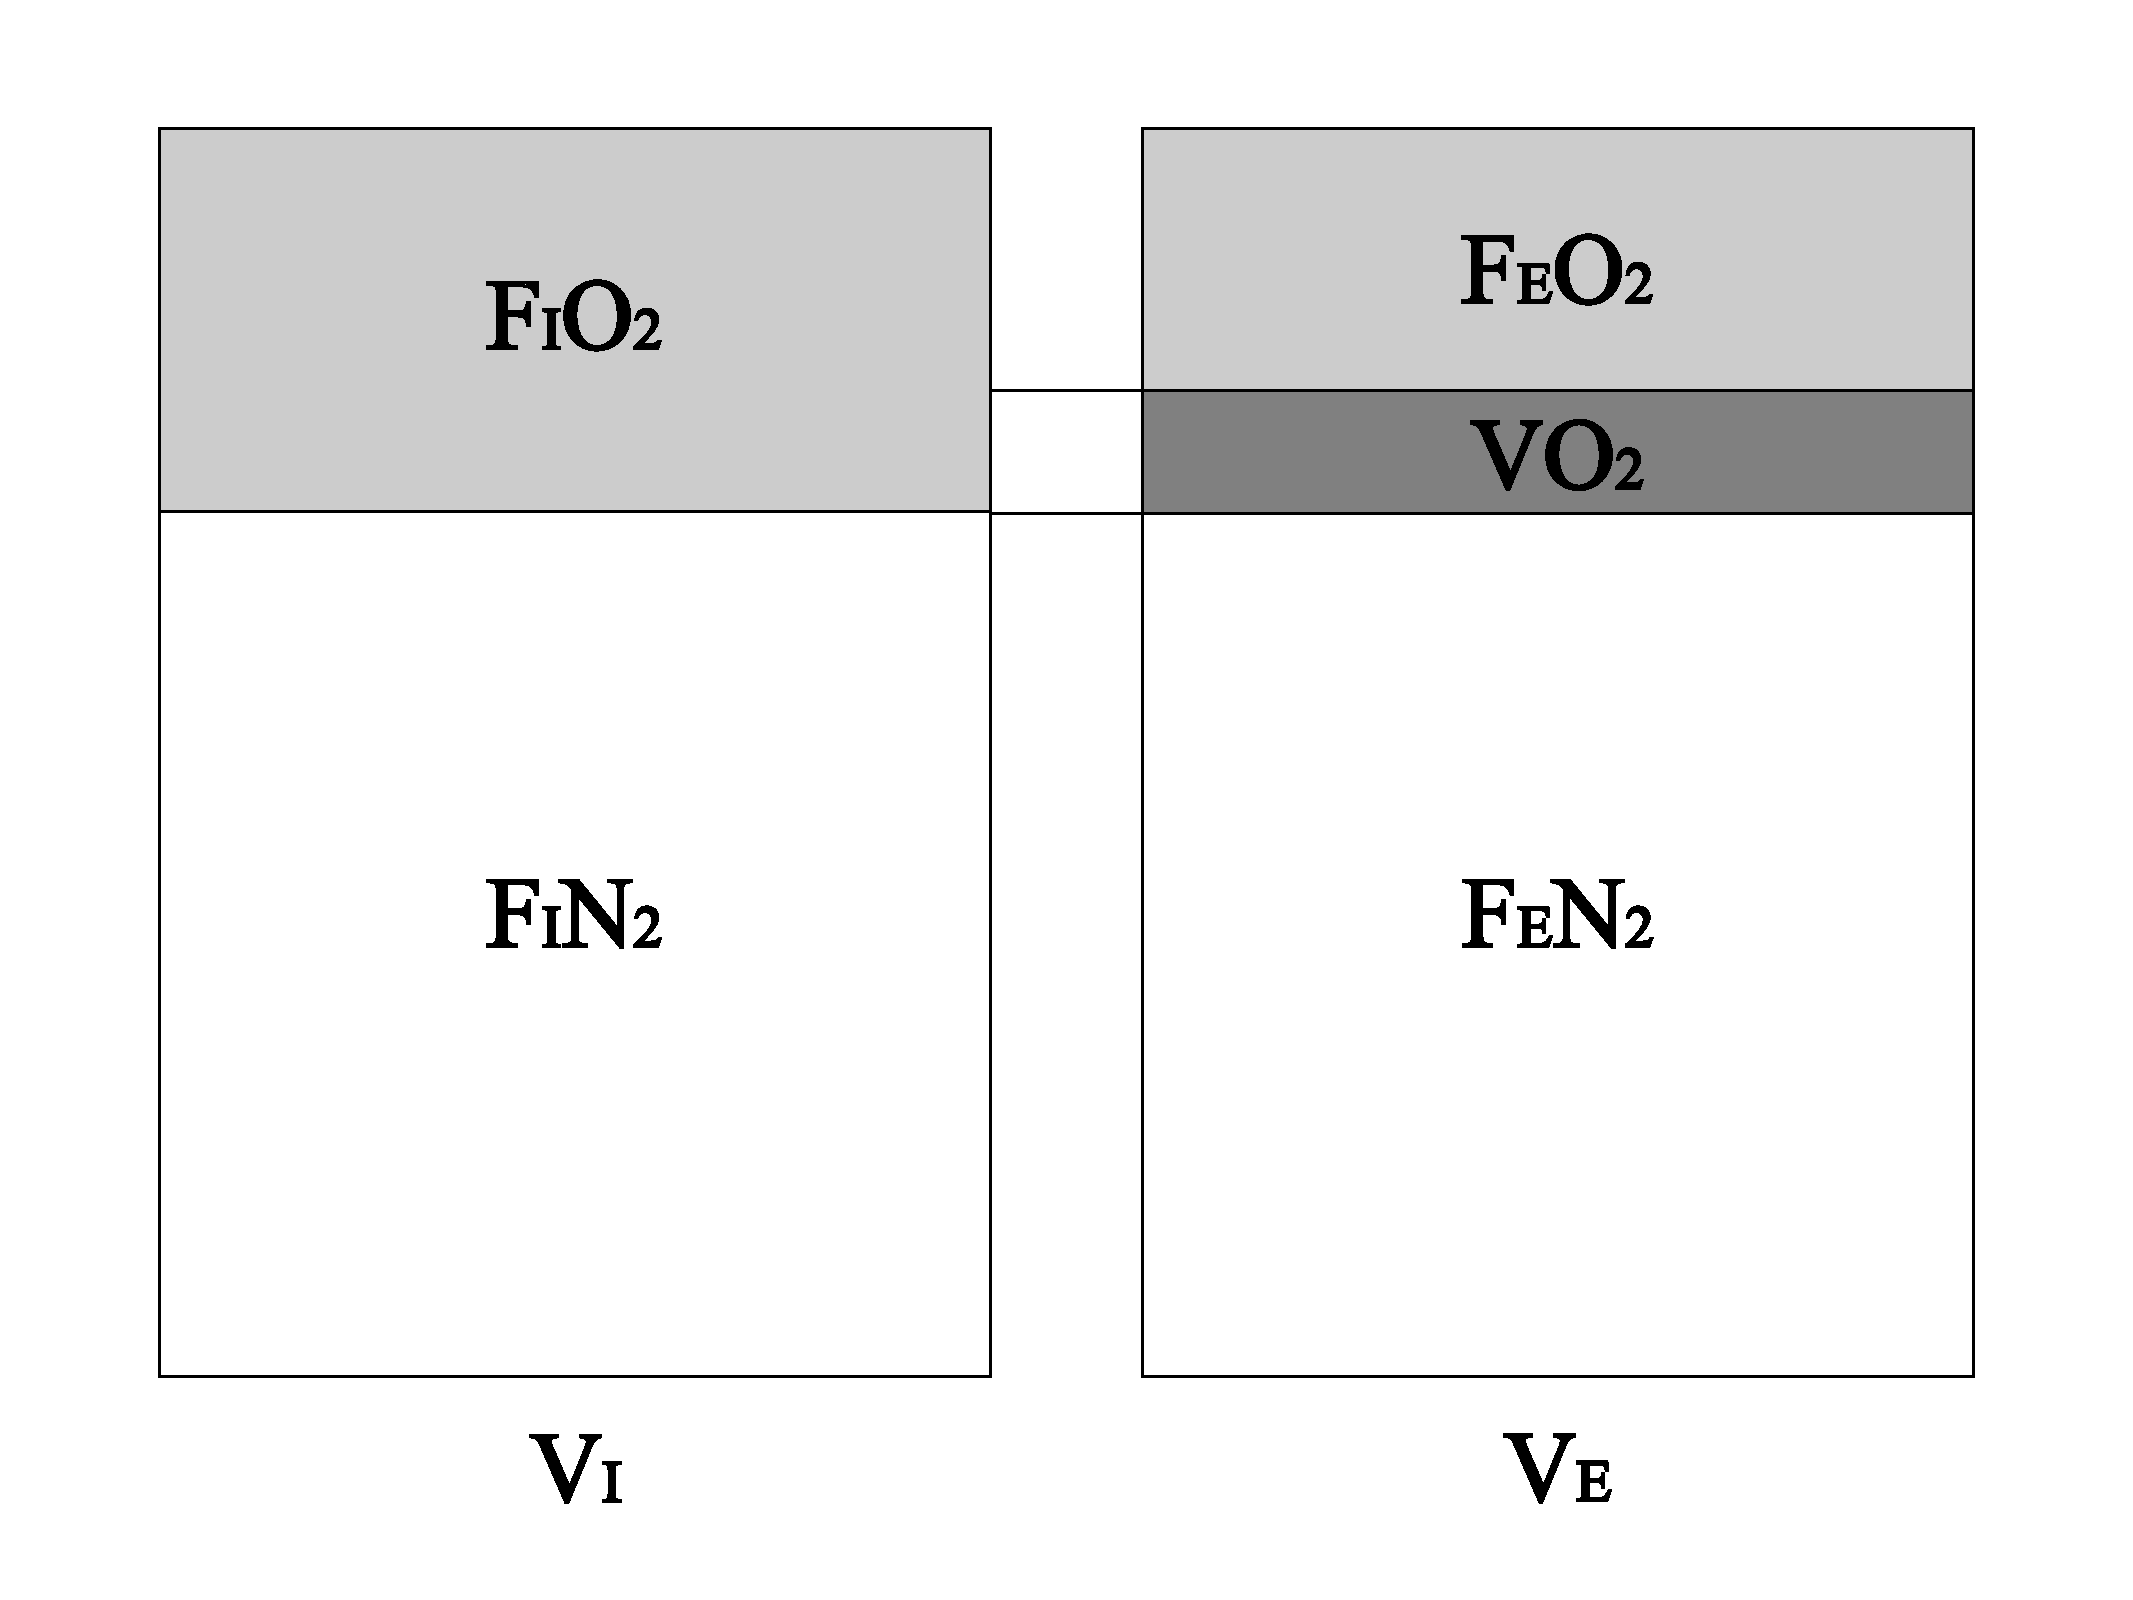
\includegraphics[width=5cm]{fig/vo2_measurement_mechanism.pdf}
    \caption{VO_2の測定}
  \end{center}
\end{figure}

このうち,吸気量V_Iは直接測定しなくても,吸気中および呼気中の窒素量から求めることが可能である.\ref{sec:n2correction}で解説する.

\subsubsection{窒素補正}
\label{sec:n2correction}

窒素は代謝に使われないため体内に吸収されない.そのため,吸気中と呼気中の窒素量は変わらないという特性を持つ(図\ref{fig:vo2_measurement_mechanism}).これを利用することで,吸気量V_Iを直接測定せずに求めることが可能である.
吸気中及び呼気中の窒素量は,吸気量または呼気量に,それぞれ吸気中の窒素濃度F_IN_2,呼気中の窒素濃度F_EN_2を掛けたものとして求められる.これと先述の窒素の特性を用いて,次の式が成り立つ.

\begin{equation}
  \label{eq:fin2fen2}
  V_I \times F_IN_2 = V_E \times F_EN_2
\end{equation}

また,この特性から呼気中の窒素濃度は,呼気中の酸素濃度F_EO_2と二酸化炭素濃度F_ECO_2を100\%から引いた残りであると考えられるから,次の式が成り立つ.

\begin{equation}
  F_EN_2 = 100 - F_EO_2 - F_ECO_2
\end{equation}

式\ref{eq:fin2fen2}をV_Iに関して変形すると

\begin{equation}
  \label{eq:vefin2fen2}
  V_I = \frac{V_E \times F_EN_2}{F_IN_2}
\end{equation}

式\ref{eq:vefin2fen2}を式\ref{eq:vo2fife}に代入すると

\begin{equation}
  \label{eq:vo2ve}
  VO_2 = \underbrace{\frac{V_E \times F_EN_2}{F_IN_2} \times F_IO_2}_{吸気中酸素量} - \underbrace{V_E \times F_EO_2}_{呼気中酸素量}
\end{equation}

式\ref{eq:vo2ve}の右辺のV_Eを括り出して整理すると

\begin{equation}
  \label{eq:n2correctformura}
  \underbrace{VO_2}_{酸素摂取量} = \underbrace{V_E}_{呼気量} \times \underbrace{\overbrace{( \frac{F_EN_2}{F_IN_2} \times F_IO_2 - F_EO_2 )}^{窒素補正}}_{酸素摂取量}
\end{equation}

式\ref{eq:n2correctformura}では,窒素は代謝に使われないため吸気中と呼気中の窒素量は変わらないという特性を利用して,吸気中の酸素濃度を呼気量に相当した酸素濃度に換算している.これを窒素補正という.

右項の酸素摂取率は,窒素補正された呼気ガス量に対する酸素濃度から,呼気中の酸素濃度を引いて得られる.
呼気中の窒素濃度は,呼気中の酸素濃度F_EO_2と二酸化炭素濃度F_ECO_2を100\%から引いた残りであると考えられるから,それらを代入すると

\begin{equation}
  VO_2 = V_E \times (\frac{100 - F_EO_2 - F_ECO_2}{F_IN_2} \times F_IO_2 - F_EO_2)
\end{equation}

通常大気中(吸気中)の窒素濃度は79.04\%,酸素濃度は20.93\%であるから,これらの値を代入して

\begin{equation}
  VO_2 = V_E \times (\frac{100 - F_EO_2 - F_ECO_2}{79.04} \times 20.93 - F_EO_2)
\end{equation}

\begin{equation}
  VO_2 = V_E \times { {100 - F_EO_2 - F_ECO_2)} \times 0.265 - F_EO_2) }
\end{equation}

以上の式から,呼気の分析から酸素摂取量を求めることができる.

\subsection{換気量(V_E)}

\subsubsection{換気量の測定}

\ref{sec:vo2}で示したように,換気量V_Eを測定するためには呼気量を測れば良い.



\subsubsection{STPD係数}
\label{sec:stpd}

呼気量から測定される換気量は,ATPS(Ambient Temperature, Pressure, Saturated with water vapor)においての値である.これは計測環境気温,計測環境気圧,水蒸気飽和における値である.酸素摂取量VO_2, 呼気中二酸化炭素量VCO2はSTPD(Standard Temperature, Pressure, Dry),0℃,1気圧の気体標準状態で表記されるため,ATPSをSTPDに換算する必要がある.この換算に使用する係数をSTPD係数と呼ぶ.STPD係数は以下の式で表される.

\begin{equation}
  \label{eq:stpd}
  STPD = \frac{P_B - P_{H2O}}{760} \times \frac{273.15}{273.15 + T}
\end{equation}

ただし,P_B: 気圧,P_{H2O}: 飽和水蒸気圧(\ref{sec:swvp}で記述する),T: 気温,273.15: 絶対温度である.

\subsubsection{飽和水蒸気圧}
\label{sec:swvp}

飽和水蒸気圧P_{H2O}は温度によって変化し,Tetens(1930)の式を用いて近似値を求めることができる.温度T[℃]の時の飽和水蒸気圧e(T)[mmHg]は次の式で求められる.

\begin{equation}
  e(T) = 6.1078 \times 10 ^ \frac{7.5T}{(T + 237.3)} \times \frac{760}{1013.25}
\end{equation}

\subsubsection{換気量の計算}

VO_2, VCO_2に使用される換気量は1分間値であるので,換気量V_{ATPS}を求めるためには呼気量Vを採気時間T[min]で割る.

\begin{equation}
  V_{ATPS} = \frac{V}{T}
\end{equation}

これにSTPD係数(\ref{eq:stpd})を掛けると換気量V_{STPD}が得られる.

\begin{equation}
  V_{STPD} = V_{ATPS} \times STPD
\end{equation}

式\ref{eq:vo2ve}より,STPD状態の吸気中酸素量V_IO_2から呼気中酸素量V_EO_2を引くことで酸素摂取量VO_2を求めることができる.

STPD状態での呼気中酸素量V_EO_2は呼気中酸素濃度F_EO2から次の式で求める.

\begin{equation}
  V_EO_2 = V_{STPD} \times \frac{F_EO2}{100}
\end{equation}

章\ref{sec:n2correction}で述べたとおり,吸気中と呼気中の窒素量は変化しない.これを利用して吸気中の窒素量からSTPD状態での吸気中酸素量V_IO_2を次の式から求める.

\begin{equation}
  V_IO_2 = V_{STPD} \times \frac{F_EN_2}{79.04} \times \frac{20.93}{100}
\end{equation}

ただし,79.04, 20.93はそれぞれ通常大気中(吸気中)の窒素濃度は79.04\%,酸素濃度は20.93\%である.

窒素補正を利用し,F_EN_2に代入すると次のようになる.

\begin{equation}
  V_IO_2 = V_{STPD} \times \frac{100 - F_EO_2 - F_ECO_2}{79.04} \times \frac{20.93}{100}
\end{equation}

通常大気中(吸気中)の窒素濃度は79.04\%,酸素濃度は20.93\%であるから,これらの値を代入して

\begin{equation}
  V_IO_2 = V_{STPD} \times \frac{100 - F_EO_2 - F_ECO_2}{79.04} \times \frac{20.93}{100}
\end{equation}

\expandafter\ifx\csname ifdraft\endcsname\relax
  \end{document}
\fi
